\subsubsection{07.04.15}
\begin{enumerate}
	
	\item The time of beginning and ending of the meeting: 16:30 - 22:10.
	
	\item Purposes of the meeting: 
	\begin{enumerate}
		
		\item Prevent the cable from leaving the reel.
		
		\item Install new servos to the MOB.
		
	\end{enumerate}

	\item Work that has been done:
	\begin{enumerate}
		
		\item We noticed the problem, that when the winch works, sometimes the cable slips over the wide reel and wraps around the axis, which slows the rising of the lift. To improve this, we installed limiters from the sides of the reel to prevent the cable from leaving it.
		\begin{figure}[H]
			\begin{minipage}[h]{0.2\linewidth}
				\center  
			\end{minipage}
			\begin{minipage}[h]{0.6\linewidth}
				\center{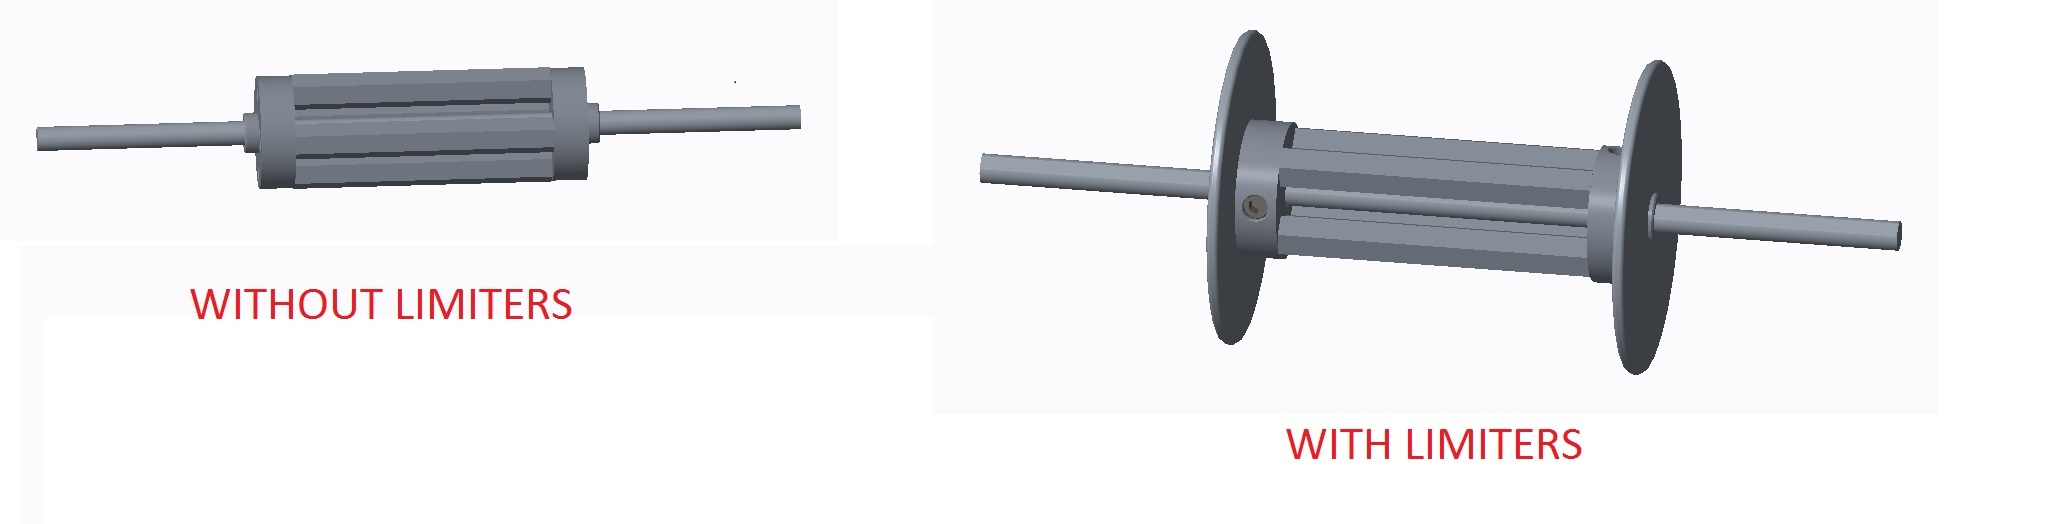
\includegraphics[scale=0.25]{days/07.04.15/images/01}}
				\caption{Improvement of the reel}
			\end{minipage}
		\end{figure}
		
		\item Also today we got 2 new strong servos and installed them to the MOB. The strong servo we used for overturning the bucket in Nederlands was left for the MCB, because this module requires less loads than the MOB, where we needed to install fresh servos. We didn't fix the servo on MCB today, because before we need to fix the MEL on the robot and next place servo in the free space.
		
	\end{enumerate}
	
	\item Results:
	\begin{enumerate}
		
		\item Limiters for the reel were installed.
		
		\item Strong servodrivers were installed.
		
	\end{enumerate}
	
	\item Tasks for the next meetings:
	\begin{enumerate}
		
		\item 
		
		\item 
		
        \item 
			
	\end{enumerate}
\end{enumerate}
\fillpage
